\documentclass[12pt,a4paper]{article}
\usepackage[utf8]{inputenc}
\usepackage[T1]{fontenc}
\usepackage{polski}
\usepackage[polish]{babel}
\usepackage{geometry}
\geometry{margin=2.5cm}
\usepackage{graphicx}
\usepackage{tabularx}
\usepackage{booktabs} 
\usepackage{hyperref}
\usepackage{bookmark}
\usepackage{enumitem}
\usepackage{titlesec}
\usepackage{microtype}
\usepackage{varwidth}
\usepackage{multicol}
\usepackage{booktabs}
\usepackage{array}
\usepackage{float}
\usepackage{listings}
\usepackage{xcolor}

\lstdefinestyle{cpp}{
    language=C++,
    basicstyle=\ttfamily\small,
    keywordstyle=\color{blue}\bfseries,
    commentstyle=\color{gray},
    stringstyle=\color{red},
    numbers=left,
    numberstyle=\tiny\color{gray},
    breaklines=true,
    frame=single,
    tabsize=4,
}
 
\usepackage{hyperref}
\hypersetup{
    colorlinks=true,
    linkcolor=black,
    urlcolor=blue,
    citecolor=black,
}

\title{
    \begin{center}
    
\includegraphics[width=\textwidth]{fig/logo.png}
    \vspace{0.25cm}
    \end{center}
    \textbf{\huge Projektowanie i analiza algorytmów} \\
    \vspace{0.5cm}
    \textit{Analiza efektywności algorytmów wyznaczania najkrótszych ścieżek w grafach}
    }
\author{Piotr Frąc}
\date{Maj 2026}



\begin{document}
\maketitle
\clearpage
\section{Wstęp}
 
Problem najkrótszej ścieżki w grafie jest jednym z fundamentalnych zagadnień
teorii grafów i informatyki. Polega on na znalezieniu połączenia między dwoma
wierzchołkami grafu ważonego, którego suma wag krawędzi jest minimalna.
Problem ten ma szerokie zastosowanie praktyczne -- od wyznaczania tras
w nawigacji GPS, przez routing pakietów w sieciach komputerowych, aż po
optymalizację logistyki i planowanie połączeń komunikacyjnych.
 
Celem niniejszego sprawozdania jest zbadanie i porównanie efektywności
dwóch algorytmów rozwiązujących ten problem: algorytmu Dijkstry oraz
algorytmu Bellmana-Forda. Analiza przeprowadzona została w zależności od
dwóch czynników: sposobu reprezentacji grafu w pamięci komputera
(lista sąsiedztwa oraz macierz sąsiedztwa) oraz gęstości grafu
(25\%, 50\%, 75\% oraz graf pełny). Eksperymenty wykonano dla grafów
o 10, 50, 100, 500 oraz 1000 wierzchołkach, a wyniki uśredniono na
podstawie 100 losowo generowanych instancji dla każdego zestawu parametrów.
 
\section{Opis struktur danych}
 
Graf jest strukturą matematyczną $G = (V, E)$, gdzie $V$ oznacza zbiór
wierzchołków, a $E$ zbiór krawędzi łączących te wierzchołki. W przypadku
grafów ważonych każda krawędź posiada dodatkowo przypisaną wartość
liczbową -- wagę. W niniejszym projekcie rozważane są grafy nieskierowane
z wagami całkowitymi z zakresu $[1, 100]$.
 
Gęstość grafu definiuje się jako stosunek liczby istniejących krawędzi
do maksymalnej możliwej liczby krawędzi. Dla grafu nieskierowanego
o $V$ wierzchołkach maksymalna liczba krawędzi wynosi $\frac{V(V-1)}{2}$,
zatem gęstość wyraża się wzorem:
 
\begin{equation}
    \rho = \frac{2|E|}{V(V-1)}
\end{equation}
 
\subsection{Lista sąsiedztwa}
 
Lista sąsiedztwa reprezentuje graf jako tablicę $V$ list, gdzie $i$-ta lista
zawiera wszystkich sąsiadów wierzchołka $i$ wraz z wagami krawędzi.
W implementacji zastosowano \texttt{std::vector<std::vector<Edge>>},
gdzie struktura \texttt{Edge} przechowuje numer docelowego wierzchołka
oraz wagę krawędzi.
 
\begin{itemize}
    \item \textbf{Złożoność pamięciowa:} $O(V + E)$
    \item \textbf{Zalety:} efektywna pamięciowo dla grafów rzadkich,
          szybkie iterowanie po sąsiadach wierzchołka $O(\deg(v))$
    \item \textbf{Wady:} wolniejszy dostęp do konkretnej krawędzi $(u, v)$
          -- wymaga przeszukania listy sąsiadów
\end{itemize}
 
\subsection{Macierz sąsiedztwa}
 
Macierz sąsiedztwa reprezentuje graf jako kwadratową macierz $V \times V$,
gdzie element matrix[i][j] przechowuje wagę krawędzi między
wierzchołkami $i$ oraz $j$, lub 0 jeśli krawędź nie istnieje.
W implementacji zastosowano \texttt{std::vector<std::vector<int>>}.
 
\begin{itemize}
    \item \textbf{Złożoność pamięciowa:} $O(V^2)$
    \item \textbf{Zalety:} dostęp do dowolnej krawędzi $(u, v)$ w czasie
          $O(1)$, prosta implementacja
    \item \textbf{Wady:} nieefektywna pamięciowo dla grafów rzadkich,
          iterowanie po sąsiadach wierzchołka zawsze kosztuje $O(V)$
          niezależnie od liczby krawędzi
\end{itemize}
 
\subsection{Porównanie reprezentacji}
 
\begin{table}[H]
    \centering
    \caption{Porównanie złożoności operacji dla obu reprezentacji}
    \begin{tabular}{lcc}
        \toprule
        \textbf{Operacja} & \textbf{Lista sąsiedztwa} & \textbf{Macierz sąsiedztwa} \\
        \midrule
        Pamięć                       & $O(V + E)$    & $O(V^2)$ \\
        Sprawdzenie krawędzi $(u,v)$ & $O(\deg(v))$  & $O(1)$   \\
        Iteracja po sąsiadach        & $O(\deg(v))$  & $O(V)$   \\
        Dodanie krawędzi             & $O(1)$        & $O(1)$   \\
        \bottomrule
    \end{tabular}
\end{table}
 
Dla grafów rzadkich (niska gęstość) lista sąsiedztwa jest zdecydowanie
bardziej efektywna. Wraz ze wzrostem gęstości różnica maleje, a dla
grafu pełnego obie reprezentacje mają porównywalną liczbę operacji
przy iteracji po sąsiadach.
 
\section{Opis algorytmów}
 
\subsection{Algorytm Dijkstry}
 
Algorytm Dijkstry rozwiązuje problem najkrótszej ścieżki od jednego
źródła do wszystkich pozostałych wierzchołków w grafie z nieujemnymi
wagami krawędzi. Został opublikowany przez Edsgera Dijkstrę w 1959 roku.
 
\subsubsection*{Idea działania}
 
Algorytm utrzymuje wektor odległości \texttt{dist[]}, gdzie
\texttt{dist[v]} oznacza aktualnie najlepiej znaną odległość od źródła
do wierzchołka $v$. Inicjalnie $\texttt{dist[src]} = 0$, a dla
pozostałych wierzchołków $\texttt{dist[v]} = \infty$. W każdej iteracji
wybierany jest wierzchołek $u$ z najmniejszą odległością spośród
jeszcze nieprzetworzonych (za pomocą kolejki priorytetowej opartej
na kopcu binarnym), a następnie wykonywana jest \textbf{relaksacja}
wszystkich krawędzi wychodzących z $u$ -- jeśli
$\texttt{dist}[u] + w(u,v) < \texttt{dist}[v]$, to \texttt{dist[v]}
jest aktualizowane.
 
\subsubsection*{Pseudokod}
 
\begin{lstlisting}[style=cpp, caption={Pseudokod algorytmu Dijkstry}]
dist[src] = 0,  dist[v] = INF  dla v != src
kolejka = {(0, src)}
 
dopoki kolejka niepusta:
    (d, u) = wyciagnij minimum z kolejki
    jesli d > dist[u]: pomin
 
    dla kazdej krawedzi (u, v, w):
        jesli dist[u] + w < dist[v]:
            dist[v] = dist[u] + w
            wstaw (dist[v], v) do kolejki
\end{lstlisting}
 
\subsubsection*{Złożoność obliczeniowa}
 
Przy zastosowaniu kolejki priorytetowej opartej na kopcu binarnym:
\begin{itemize}
    \item każdy wierzchołek jest wyciągany z kolejki co najwyżej raz:
          $O(V \log V)$
    \item każda krawędź powoduje co najwyżej jedno wstawienie do kolejki:
          $O(E \log V)$
    \item łącznie: $\mathbf{O((V + E) \log V)}$
\end{itemize}
 
\textbf{Ograniczenie:} algorytm nie działa poprawnie dla grafów
z ujemnymi wagami krawędzi, ponieważ zakłada że po wyciągnięciu
wierzchołka z kolejki jego odległość jest już ostateczna.
 
\subsection{Algorytm Bellmana-Forda}
 
Algorytm Bellmana-Forda również rozwiązuje problem najkrótszej ścieżki
od jednego źródła, ale dopuszcza ujemne wagi krawędzi. Nie może jednak
działać poprawnie gdy w grafie istnieje cykl o ujemnej sumie wag.
 
\subsubsection*{Idea działania}
 
Algorytm wykonuje $V - 1$ rund relaksacji wszystkich krawędzi grafu.
Wynika to z faktu że najkrótsza ścieżka w grafie o $V$ wierzchołkach
może zawierać co najwyżej $V - 1$ krawędzi (zakładając brak ujemnych
cykli). Po każdej rundzie gwarantowane jest że znane są optymalne
ścieżki używające co najwyżej $k$ krawędzi, gdzie $k$ to numer rundy.
 
\subsubsection*{Pseudokod}
 
\begin{lstlisting}[style=cpp, caption={Pseudokod algorytmu Bellmana-Forda}]
dist[src] = 0,  dist[v] = INF  dla v != src
 
powtorz V-1 razy:
    dla kazdego wierzcholka u:
        jesli dist[u] = INF: pomin
        dla kazdej krawedzi (u, v, w):
            jesli dist[u] + w < dist[v]:
                dist[v] = dist[u] + w
\end{lstlisting}
 
\subsubsection*{Złożoność obliczeniowa}
 
\begin{itemize}
    \item zewnętrzna pętla wykonuje się $V - 1$ razy
    \item wewnętrzna iteruje po wszystkich krawędziach: $O(E)$
    \item łącznie: $\mathbf{O(V \cdot E)}$
\end{itemize}
 
Dla grafu pełnego gdzie $E = \frac{V(V-1)}{2}$ złożoność wynosi $O(V^3)$,
co czyni algorytm znacznie wolniejszym od Dijkstry dla dużych gęstych grafów.
 
\section{Metodyka eksperymentów}
 
\subsection{Środowisko testowe}
 
Eksperymenty przeprowadzono na komputerze z systemem Linux. Program
napisano w języku C++17 i skompilowano kompilatorem \texttt{g++}
z flagą optymalizacji \texttt{-O2}. Do pomiaru czasu użyto
\texttt{std::chrono::steady\_clock} z rozdzielczością nanosekund.
 
\subsection{Generowanie grafów}
 
Grafy generowano losowo z zadaną gęstością. Dla każdej pary wierzchołków
$(i, j)$ gdzie $i < j$ losowano liczbę z zakresu $[1, 100]$ - jeśli
była ona mniejsza lub równa zadanemu procentowi gęstości, krawędź była
dodawana z losową wagą całkowitą z zakresu $[1, 100]$. Takie podejście
zapewnia że oczekiwana gęstość grafu jest równa zadanemu parametrowi,
a krawędzie są rozłożone równomiernie. Do generowania liczb losowych
użyto generatora Mersenne Twister (\texttt{std::mt19937}).
 
\subsection{Parametry eksperymentów}
 
Badania przeprowadzono dla następujących parametrów:
 
\begin{table}[H]
    \centering
    \caption{Parametry eksperymentów}
    \begin{tabular}{ll}
        \toprule
        \textbf{Parametr} & \textbf{Wartości} \\
        \midrule
        Liczba wierzchołków $V$ & 10, 50, 100, 500, 1000 \\
        Gęstość grafu           & 25\%, 50\%, 75\%, 100\% \\
        Reprezentacja grafu     & lista sąsiedztwa, macierz sąsiedztwa \\
        Algorytmy               & Dijkstra, Bellman-Ford \\
        Liczba instancji        & 100 \\
        \bottomrule
    \end{tabular}
\end{table}
 
Łącznie wygenerowano i zbadano
$5 \times 4 \times 2 \times 2 \times 100 = 8000$ instancji.
 
\subsection{Sposób pomiaru}
 
Dla każdej instancji mierzono osobno czas wykonania algorytmu Dijkstry
i Bellmana-Forda na tym samym grafie. Czas generowania grafu był wyłączony
z pomiaru - mierzono wyłącznie czas wykonania algorytmu od momentu
przekazania gotowego grafu do momentu zwrócenia wektora odległości.
Wyniki 100 przebiegów dla każdego zestawu parametrów uśredniono
arytmetycznie i przedstawiono w tabelach oraz na wykresach.
 
\section{Wyniki i analiza}
 
 
 
\subsection{Tabele uśrednionych czasów wykonania}
 
Poniższe tabele przedstawiają średnie czasy wykonania (w mikrosekundach) dla każdego algorytmu
i reprezentacji grafu, uśrednione po 100 losowych instancjach.
 
\begin{table}[H]
\centering
\caption{Dijkstra -- lista sąsiedztwa [$\mu$s]}
\begin{tabular}{rrrrr}
\toprule
\textbf{V} & \textbf{25\%} & \textbf{50\%} & \textbf{75\%} & \textbf{100\%} \\
\midrule
10   & 2,57    & 4,72    & 4,88    & 5,50    \\
50   & 37,59   & 48,38   & 58,27   & 62,25   \\
100  & 102,71  & 132,44  & 150,52  & 167,68  \\
500  & 1073,32 & 1367,78 & 1675,62 & 1970,00 \\
1000 & 2864,11 & 4010,74 & 5134,06 & 6203,25 \\
\bottomrule
\end{tabular}
\end{table}
 
\begin{table}[H]
\centering
\caption{Dijkstra -- macierz sąsiedztwa [$\mu$s]}
\begin{tabular}{rrrrr}
\toprule
\textbf{V} & \textbf{25\%} & \textbf{50\%} & \textbf{75\%} & \textbf{100\%} \\
\midrule
10   & 3,93     & 6,93     & 9,26     & 9,35     \\
50   & 66,91    & 93,86    & 108,32   & 117,13   \\
100  & 207,21   & 295,53   & 326,18   & 352,30   \\
500  & 3019,12  & 4633,74  & 5023,63  & 5551,72  \\
1000 & 10415,25 & 16601,80 & 18216,97 & 19424,43 \\
\bottomrule
\end{tabular}
\end{table}
 
\begin{table}[H]
\centering
\caption{Bellman-Ford -- lista sąsiedztwa [$\mu$s]}
\begin{tabular}{rrrrr}
\toprule
\textbf{V} & \textbf{25\%} & \textbf{50\%} & \textbf{75\%} & \textbf{100\%} \\
\midrule
10   & 5,09       & 7,15       & 8,22       & 9,51       \\
50   & 261,61     & 386,43     & 517,32     & 621,50     \\
100  & 1543,04    & 2537,45    & 3509,35    & 4480,62    \\
500  & 144347,86  & 271842,33  & 401145,01  & 524243,30  \\
1000 & 1091861,07 & 2102768,87 & 3119690,34 & 4148643,49 \\
\bottomrule
\end{tabular}
\end{table}
 
\begin{table}[H]
\centering
\caption{Bellman-Ford -- macierz sąsiedztwa [$\mu$s]}
\begin{tabular}{rrrrr}
\toprule
\textbf{V} & \textbf{25\%} & \textbf{50\%} & \textbf{75\%} & \textbf{100\%} \\
\midrule
10   & 14,87       & 27,26        & 39,02        & 39,85        \\
50   & 1574,27     & 2380,51      & 2825,33      & 3038,05      \\
100  & 11030,05    & 17490,15     & 19774,89     & 21245,72     \\
500  & 1116061,02  & 1870909,78   & 2061749,11   & 2256237,05   \\
1000 & 8517761,25  & 14557804,55  & 15991939,04  & 16963052,35  \\
\bottomrule
\end{tabular}
\end{table}
 
\subsection{Wykresy Typ 1 -- osobne dla każdej reprezentacji}
 
Wykresy poniżej przedstawiają czas wykonania w funkcji liczby wierzchołków,
dla obu algorytmów i wszystkich gęstości, osobno dla każdej reprezentacji grafu.
 
\begin{figure}[H]
    \centering
    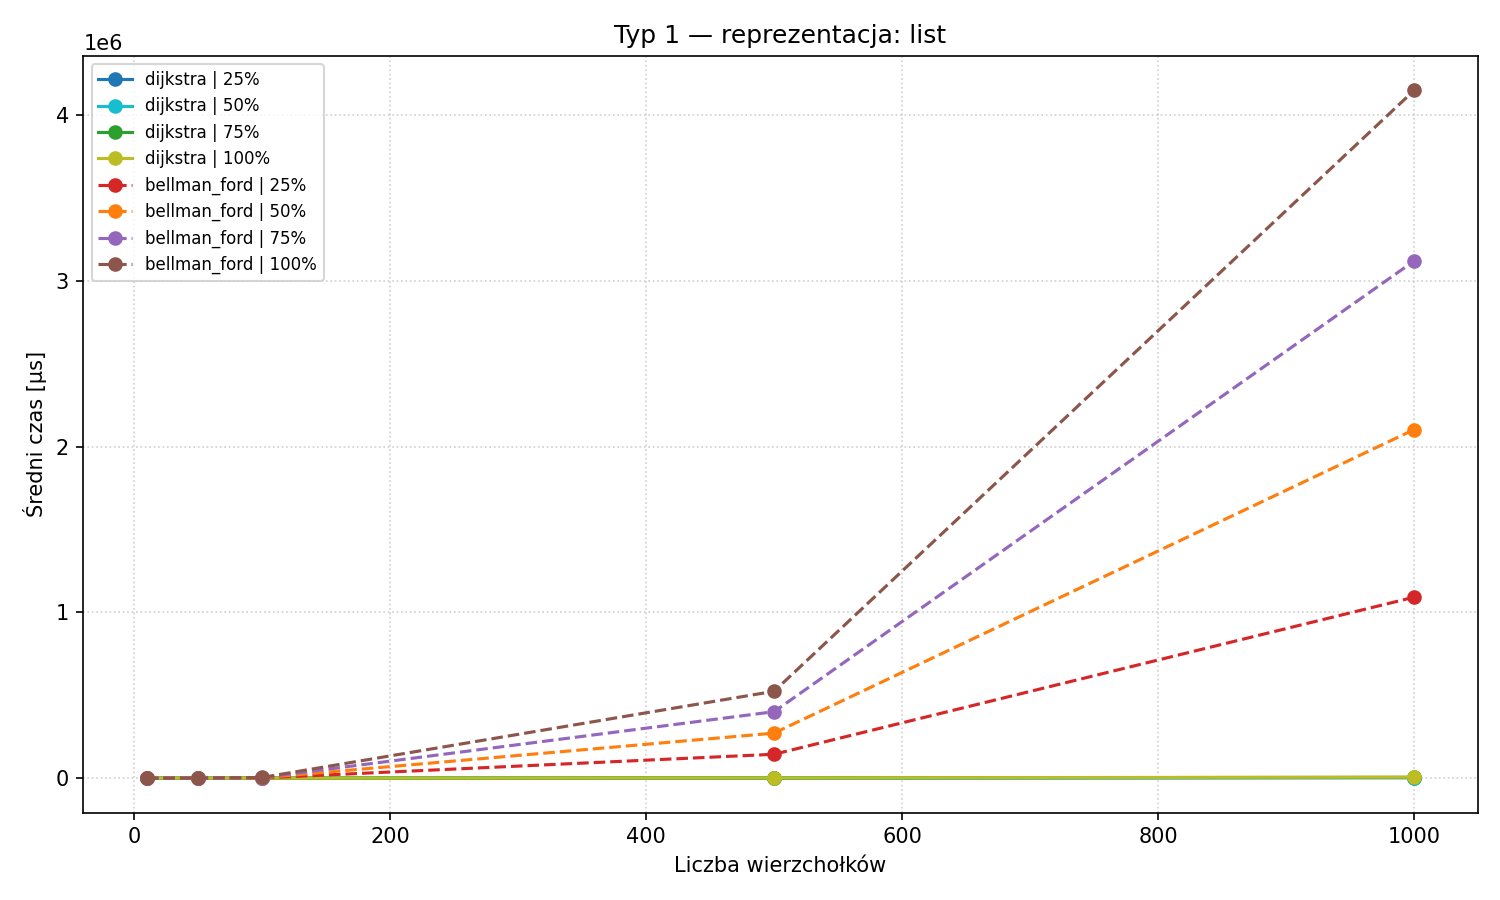
\includegraphics[width=0.92\textwidth]{../data/typ1_list.png}
    \caption{Typ 1 -- reprezentacja listowa}
\end{figure}
 
\begin{figure}[H]
    \centering
    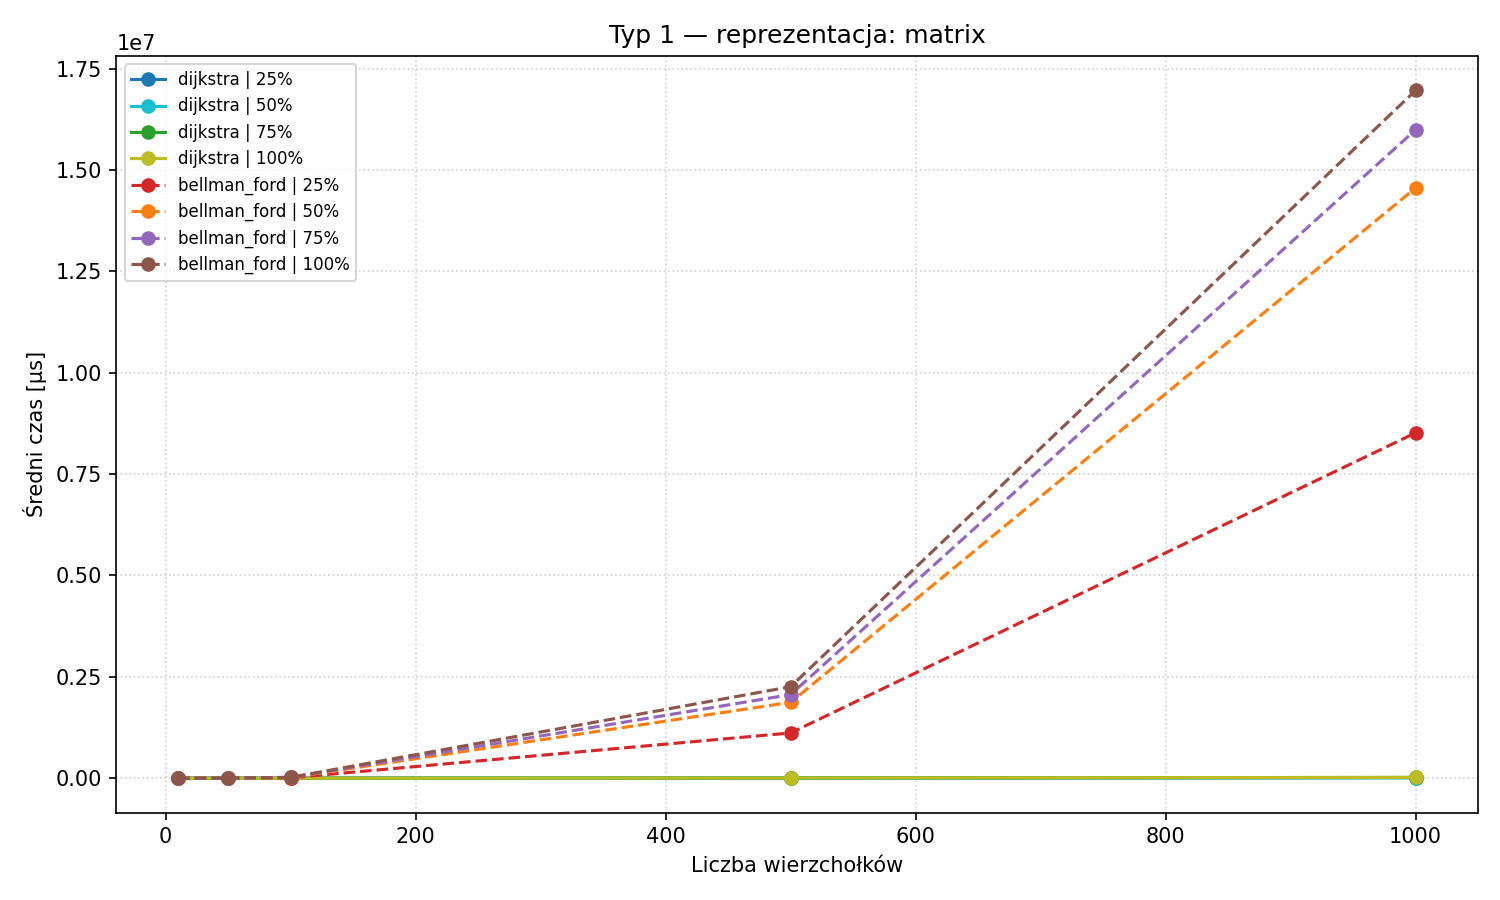
\includegraphics[width=0.92\textwidth]{../data/typ1_matrix.png}
    \caption{Typ 1 -- reprezentacja macierzowa}
\end{figure}
 
Na obu wykresach wyraźnie widać przewagę algorytmu Dijkstry -- jego linie (ciągłe)
pozostają bliskie zeru w porównaniu z Bellmanem-Fordem (przerywane), który rośnie
gwałtownie dla $V \geq 500$. Bellman-Ford jest znacznie wolniejszy, co jest szczególnie
widoczne na reprezentacji macierzowej -- dla grafu pełnego z 1000 wierzchołków osiąga
czas rzędu $1{,}7 \times 10^7\ \mu$s, czyli około 17 sekund, podczas gdy Dijkstra
na tej samej reprezentacji potrzebuje zaledwie $19424\ \mu$s.
 
\subsection{Wykresy Typ 2 -- osobne dla każdej gęstości}
 
\begin{figure}[H]
    \centering
    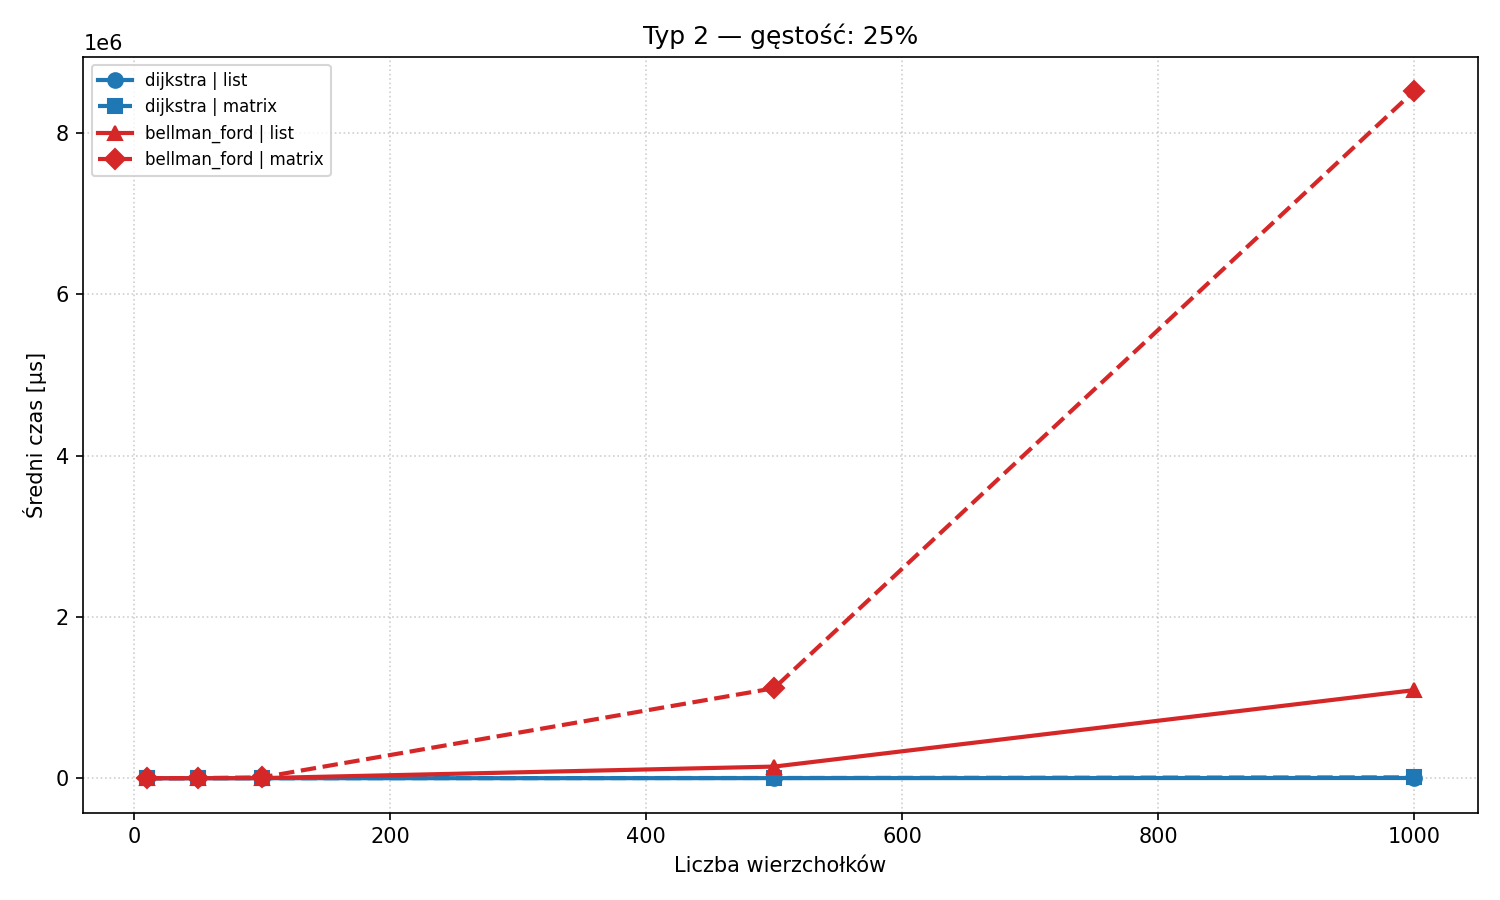
\includegraphics[width=0.92\textwidth]{../data/typ2_25.png}
    \caption{Typ 2 -- gęstość 25\%}
\end{figure}
 
\begin{figure}[H]
    \centering
    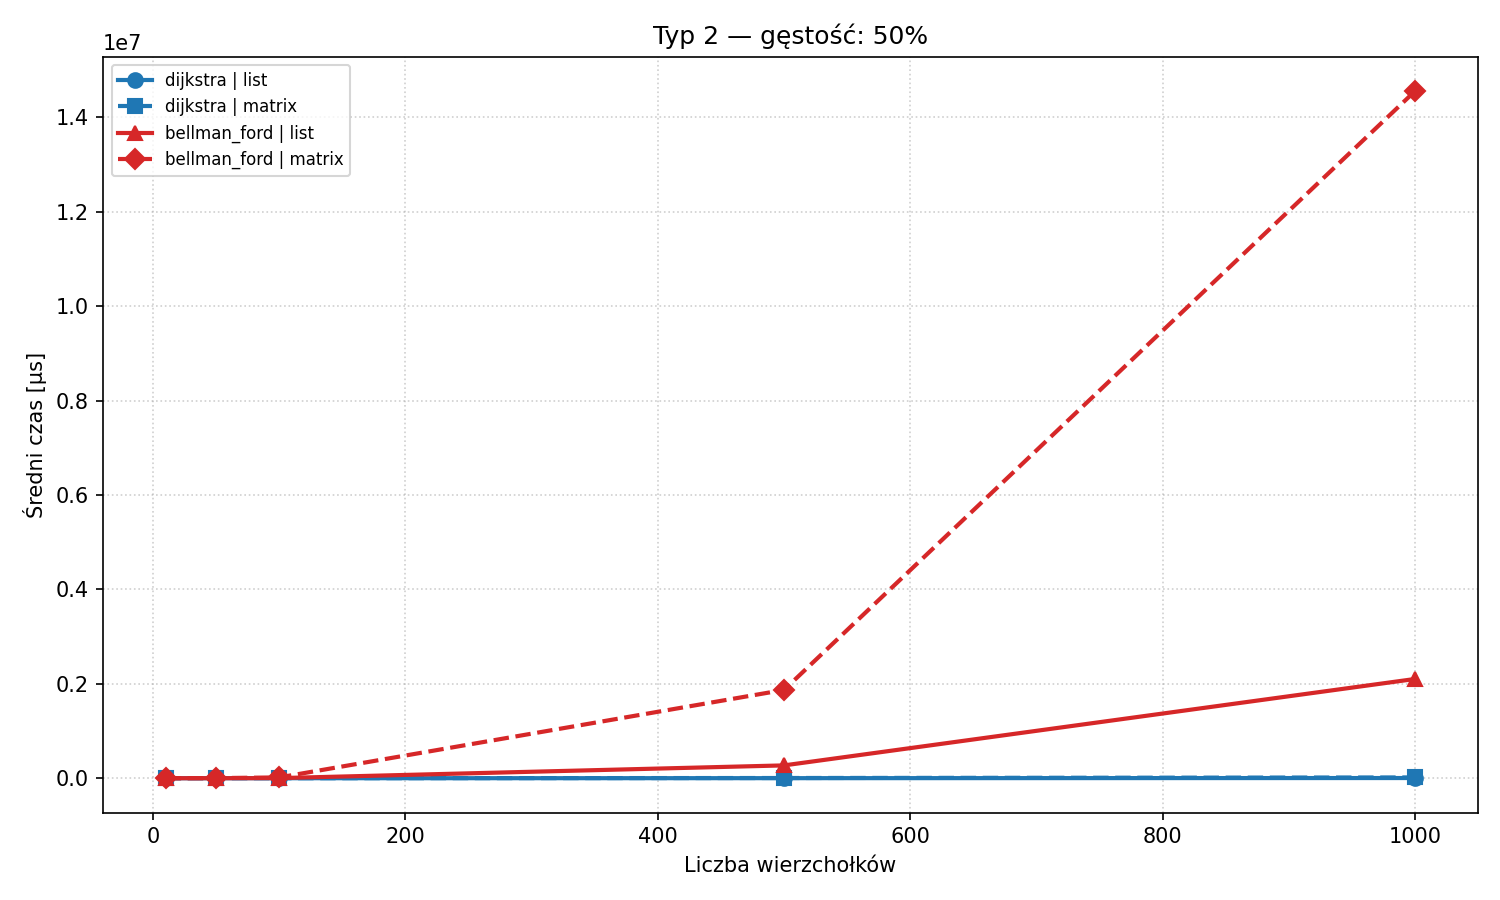
\includegraphics[width=0.92\textwidth]{../data/typ2_50.png}
    \caption{Typ 2 -- gęstość 50\%}
\end{figure}
 
\begin{figure}[H]
    \centering
    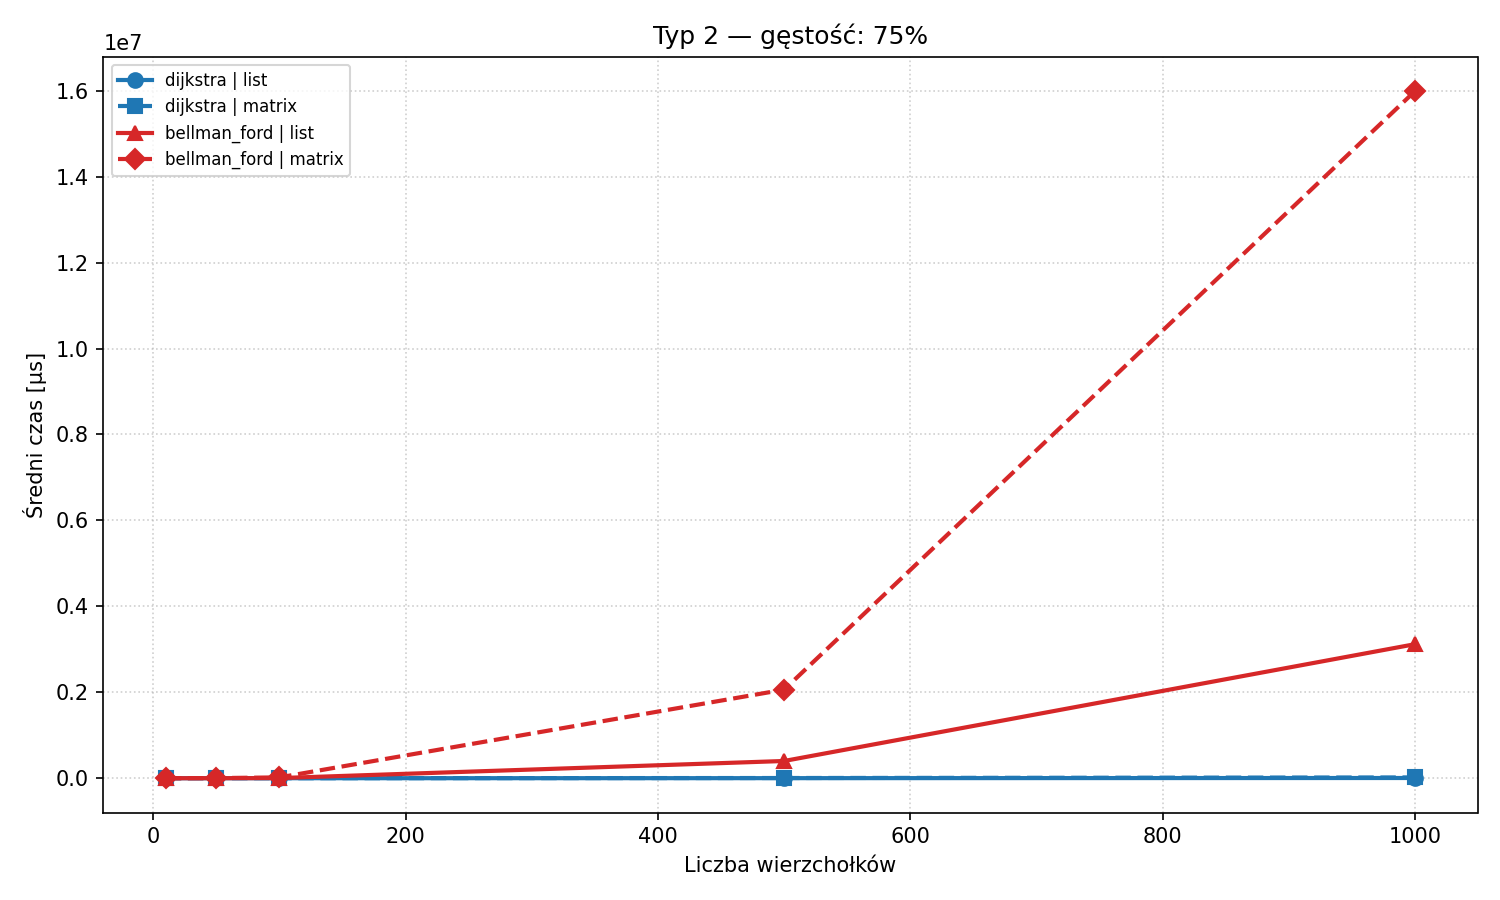
\includegraphics[width=0.92\textwidth]{../data/typ2_75.png}
    \caption{Typ 2 -- gęstość 75\%}
\end{figure}
 
\begin{figure}[H]
    \centering
    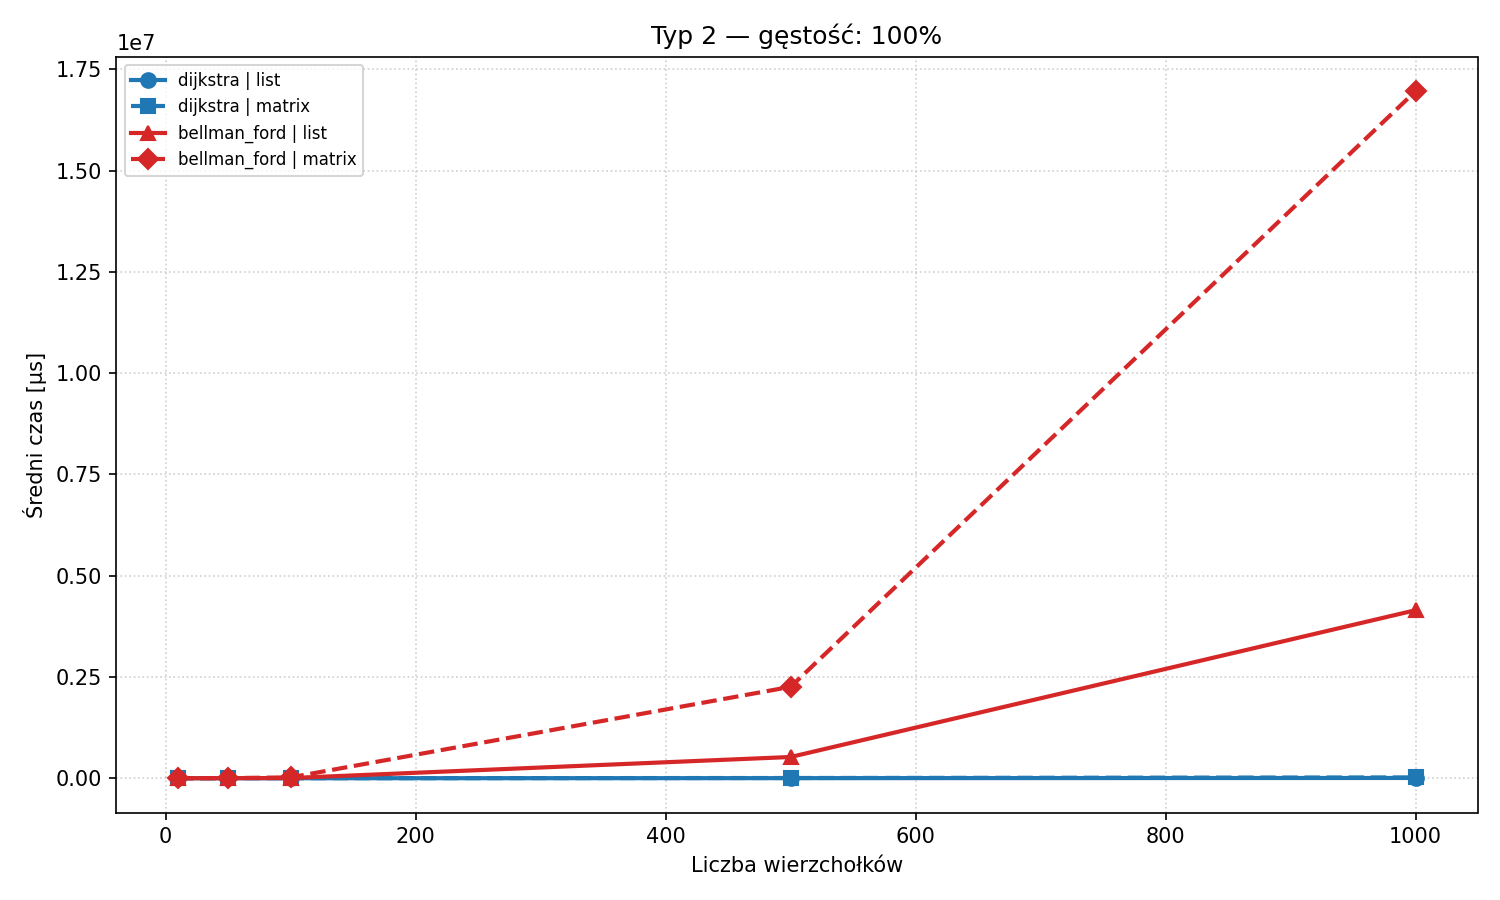
\includegraphics[width=0.92\textwidth]{../data/typ2_100.png}
    \caption{Typ 2 -- gęstość 100\% (graf pełny)}
\end{figure}
 
Na wykresach Typ 2 widać że Dijkstra (niebieski) jest wielokrotnie szybszy od Bellmana-Forda
(czerwony) niezależnie od gęstości grafu. Wraz ze wzrostem gęstości różnica między
reprezentacjami dla Bellmana-Forda staje się coraz bardziej widoczna -- macierz (przerywana)
jest wyraźnie wolniejsza od listy (ciągła). Dijkstra natomiast jest na tyle szybki,
że obie jego reprezentacje zlewają się przy dole osi Y.
 
\subsection{Wykresy osobne dla każdego algorytmu}
 
\begin{figure}[H]
    \centering
    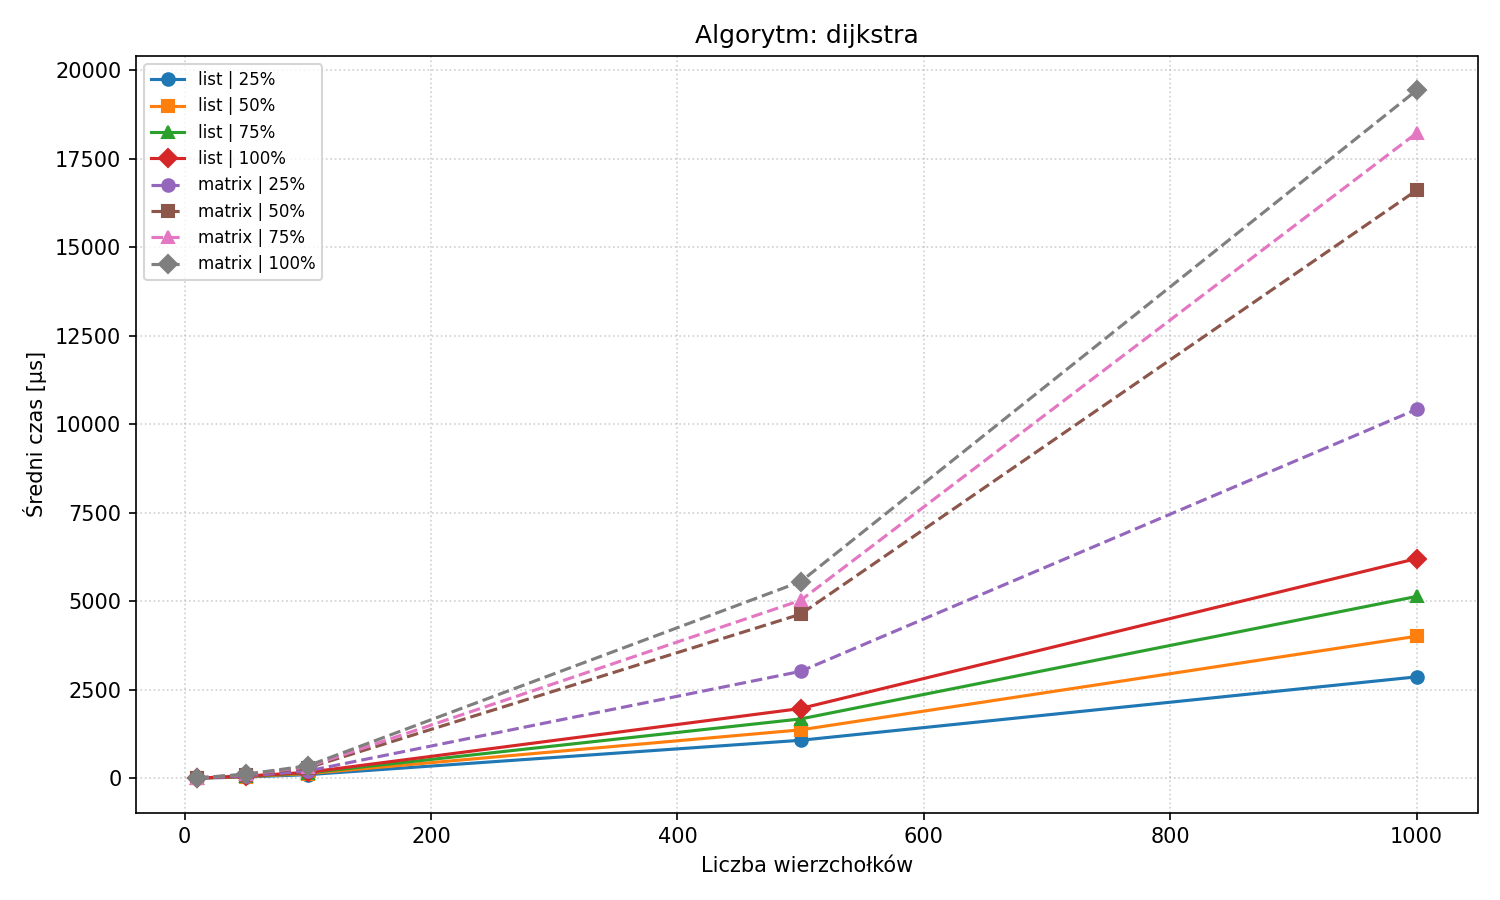
\includegraphics[width=0.92\textwidth]{../data/algo_dijkstra.png}
    \caption{Algorytm Dijkstry -- porównanie reprezentacji i gęstości}
\end{figure}
 
\begin{figure}[H]
    \centering
    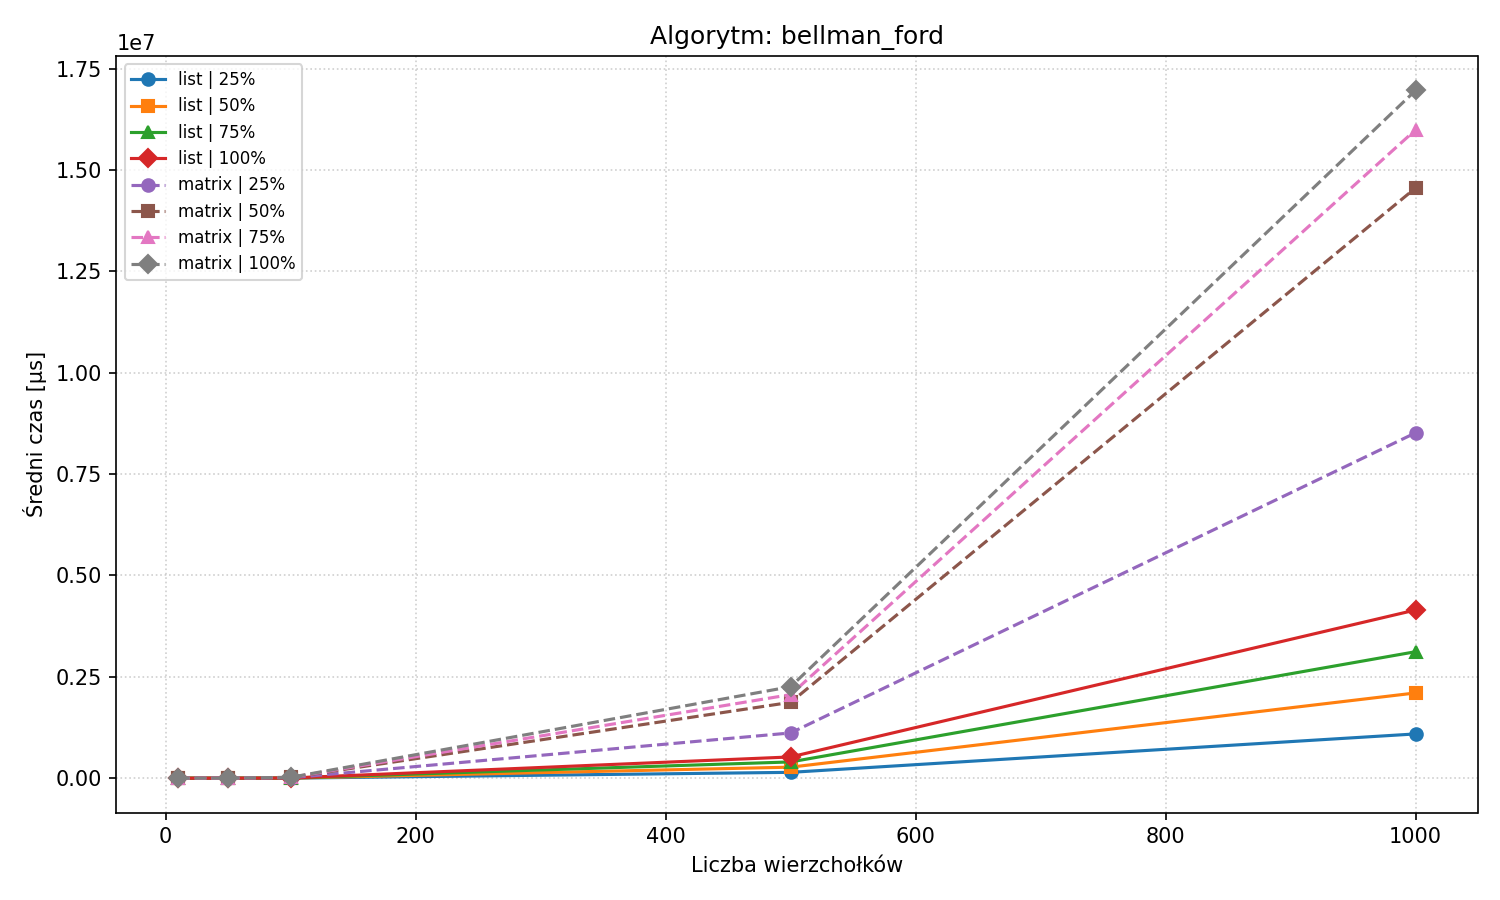
\includegraphics[width=0.92\textwidth]{../data/algo_bellman_ford.png}
    \caption{Algorytm Bellmana-Forda -- porównanie reprezentacji i gęstości}
\end{figure}
 
Wykres Dijkstry pokazuje że macierz sąsiedztwa jest konsekwentnie wolniejsza od listy
dla wszystkich gęstości -- przy 1000 wierzchołkach różnica wynosi około 3-krotność
(macierz 100\%: $19424\ \mu$s, lista 100\%: $6203\ \mu$s). Wzrost czasu wraz z gęstością
jest wyraźny ale umiarkowany -- Dijkstra dobrze radzi sobie nawet z gęstymi grafami.
 
Wykres Bellmana-Forda ujawnia dramatyczną różnicę między reprezentacjami.
Macierz sąsiedztwa jest wielokrotnie wolniejsza od listy -- przy 1000 wierzchołkach
i gęstości 25\% wynosi to blisko 8-krotność ($8\,517\,761\ \mu$s vs $1\,091\,861\ \mu$s).
Wynika to z faktu że w macierzy iteracja po sąsiadach wierzchołka kosztuje zawsze $O(V)$,
niezależnie od faktycznej liczby krawędzi, co przy $V-1$ rundach Bellmana-Forda
kumuluje się do $O(V^3)$ operacji.
 
\section{Wnioski}
 
Przeprowadzone eksperymenty potwierdzają teoretyczne przewidywania dotyczące
złożoności obliczeniowej obu algorytmów.
 
\textbf{Dijkstra vs Bellman-Ford.}
Algorytm Dijkstry jest wielokrotnie szybszy od Bellmana-Forda dla grafów
z nieujemnymi wagami. Przy 1000 wierzchołkach i grafie pełnym Dijkstra
na liście sąsiedztwa potrzebuje średnio $6203\ \mu$s, podczas gdy
Bellman-Ford na tej samej reprezentacji potrzebuje $4\,148\,643\ \mu$s --
jest to około 670-krotna różnica. Wynika to bezpośrednio z różnicy
złożoności: $O((V+E)\log V)$ dla Dijkstry wobec $O(V \cdot E)$ dla
Bellmana-Forda.
 
\textbf{Wpływ reprezentacji grafu.}
Dla algorytmu Dijkstry lista sąsiedztwa jest konsekwentnie szybsza od
macierzy sąsiedztwa -- przy 1000 wierzchołkach i pełnym grafie lista jest
około 3 razy szybsza. Wynika to z faktu że lista pozwala iterować tylko
po faktycznych sąsiadach ($O(\deg(v))$), podczas gdy macierz wymaga
przejrzenia całego wiersza ($O(V)$).
 
Dla algorytmu Bellmana-Forda różnica jest jeszcze bardziej dotkliwa.
Macierz sąsiedztwa jest przy 1000 wierzchołkach i gęstości 25\%
blisko 8 razy wolniejsza od listy. Dla rzadkich grafów lista przetwarza
tylko istniejące krawędzie, natomiast macierz zawsze wykonuje $V^2$
sprawdzeń w każdej rundzie.
 
\textbf{Wpływ gęstości grafu.}
Wraz ze wzrostem gęstości rośnie czas wykonania obu algorytmów, co jest
zgodne z teorią -- więcej krawędzi oznacza więcej operacji. Wzrost jest
bardziej stromy dla Bellmana-Forda ze względu na jego wyższą złożoność.
Dla Dijkstry wzrost czasu z 25\% do 100\% gęstości jest umiarkowany
i akceptowalny praktycznie.
 
\textbf{Zgodność z teorią.}
Uzyskane wyniki są zgodne z przewidywaniami teoretycznymi. Jedyna
pozorna anomalia -- linie Dijkstry na listowej reprezentacji wyglądające
na prawie zerowe w porównaniu do Bellmana-Forda -- wynika wyłącznie
ze skali osi Y, która musi pomieścić bardzo duże wartości Bellmana-Forda.
W osobnym wykresie Dijkstry widać że jego czas rośnie prawidłowo wraz
z $V$ i gęstością.
 

\end{document}